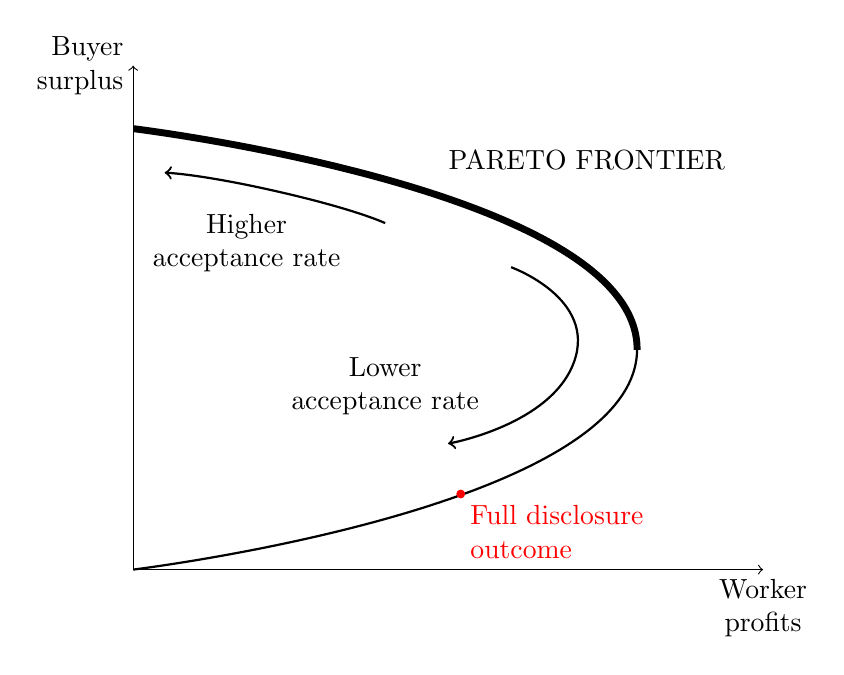
\begin{tikzpicture}[xscale=.8,yscale=.8] 

		\draw [<->] (0,8) node (yaxis)[left,align=right] {Buyer\\ surplus} 
		        |- (10,0) node (xaxis) [below,align=center] {Worker\\ profits};
	\def\mycoordinates{(0,0) (8,3.5) (0,7)}

	%\draw[step=1cm,gray,very thin] (0,0) grid (10,8);

	\def\mycoordinates{(0,0) (8,3.5) (0,7)}

	\draw[thick] plot [smooth,tension=1.3] coordinates {\mycoordinates};
	\begin{scope}
	    \clip (0,3.5) rectangle (10,8);
	    \draw [line width=2.5] plot [smooth,tension=1.3] coordinates {\mycoordinates};
	  \end{scope}

	

	\draw[thick,->] plot [smooth,tension=1.3] coordinates {(4,5.5)  (2.3,6) (.5,6.3)};

	\draw[thick,->] plot [smooth,tension=1.3] coordinates {(6,4.8) (7,3.3) (5,2)};



	\node at (7.2,6.2) [above] {PARETO FRONTIER};


	\node at (1.8,5.8) [below,align=center] {Higher\\ acceptance rate};

	\node at (4,2.3) [above,align=center] {Lower\\ acceptance rate};


	\coordinate (A) at (5.2,1.2);
        \fill[red] (A)  circle (2pt) ;
	\node at (5.2,.6) [right,red,align=left] {Full disclosure\\ outcome};




        
\end{tikzpicture}